% This is samplepaper.tex, a sample chapter demonstrating the
% LLNCS macro package for Springer Computer Science proceedings;
% Version 2.20 of 2017/10/04
%
\documentclass[runningheads]{llncs}
\usepackage{amsmath}
\usepackage{hyperref}
%
\usepackage{graphicx}
\pagestyle{headings}
\setcounter{tocdepth}{5}
% Used for displaying a sample figure. If possible, figure files should
% be included in EPS format.
%
% If you use the hyperref package, please uncomment the following line
% to display URLs in blue roman font according to Springer's eBook style:
% \renewcommand\UrlFont{\color{blue}\rmfamily}

\begin{document}
%
\title{Distributed Teams Are Founded on Explicit
Communication Channels}
%
%\titlerunning{Abbreviated paper title}
% If the paper title is too long for the running head, you can set
% an abbreviated paper title here
%
\author{Het Jatin Dalal}
%

%
\institute{Computer Science and Software Engineering , Concordia University \\ 
\vspace{10pt}  VCS: Github: \href{https://github.com/Het95/40200513-SOEN6481-TAS}{https://github.com/Het95/40200513-SOEN6481-TAS}}

%
%
\maketitle              % typeset the header of the contribution
%
{\def\addcontentsline#1#2#3{}\maketitle}


\begin{abstract}
    An increase in team size makes it harder to communicate effectively across floors, rooms, cities, or even separate geographical areas. The increased usage of explicit communication channels has thereby improved productivity as well as a number of other aspects of working in a distributed team environment. A team can manage and develop more quickly if written communication is taken into consideration. It also explains how several forms of communication—synchronous, asynchronous, or a mix of the two—are needed to share resources, fill in knowledge gaps, and handle urgent matters. 
    
    \keywords{Explicit communication \and information gaps \and Synchronous \and Ashyncronous \and Distributed team}
    \end{abstract}
    %
    %
    %
    \tableofcontents
    \newpage

    \section{Introduction}
    \subsection{Motivation}

    \begin{figure}   
        
\includegraphics[width=0.2\linewidth]{DTlogo.png}
    \end{figure}

    The motivation for researching "Distributed Teams Established on Explicit Defined Communication Channels" stems from a number of key considerations and the difficulties of modern work contexts.
    
    \begin{enumerate}
        \item \textbf{Surge in popularity of Distributed Team}: The majority of businesses with growing workforces are shifting to distributed team structure, particularly in light of recent pandemics like COVID-19. This makes it much more important in such an environment to collaborate and communicate effectively.~\cite{refbook1} 
        \item \textbf{Accountability}: Having clear channels of communication within the team facilitates awareness of individual roles and responsibilities.~\cite{refbook1}
        \item \textbf{Collaboration}: Distributed teams can share project-related materials and do various other project management tasks with each other when they have clear communication channels.~\cite{refbook1}
        \item \textbf{Embrace, Evolve, Adjust}: One must adjust to the changing environment due to changes in new technology, team and company sizes, and the organization can concentrate more on this by employing clear communication channels.~\cite{refbook1}
    \end{enumerate}
    
    \subsection{Problem Statement} In distributed team environment, the challenge of effective in-person communication has emerged due to its larger size. Interruptions for resource retrieval are also causing productivity loss, especially when team members are intently focused. The necessity for well-defined communication channels has evolved, accompanied by disputes over the advantages of synchronous versus asynchronous systems. There is a need to build a culture of written communication and to decisively identify and implement clear and effective communication channels in distributed team environment in order to unlock quick growth and better productivity.~\cite{refbook1}

    \subsection{Objectives} In this investigation, the key objective of the analysis is to describe the significance of using clear and explicit communication channels within distant work environments to boost productivity, efficiency, reducing interruptions, fill information gaps while also allowing them to grow faster. The ultimate objective is to elevate team performance to a new level, promote alignment, preparing teams to work remotely and build resilient teams that can adjust to change.This will help to simplify project management, particularly when adding new team members, and will be advantageous to managers, team leaders, and team members alike. ~\cite{refbook1}

    \section{Background Material}
For the context of the report, it is important to know all the following terms in order to gain proper understanding.

 \begin{itemize}
    \item \textbf{Distributed/Remote Teams}: The Distributed Team is spread over the same rooms, city, and possibly even continent. In a nutshell, it consists of two or more people who do not share the same physical workspace or geographical location.~\cite{refbook1}\\
    \item \textbf{Communication Challenges}: Team members' productivity may suffer if they are unclear about where to obtain information or how to communicate well. They could squander time attempting to find information or cause their teammates needless disruptions. causing tap on the shoulder or chat app notifications, when working in deep focus mode ~\cite{refbook1}\\
    \item \textbf{Synchronous and Asynchronous communication channels}: 
    Synchronous communication channels, which primarily include voice messages, video conferencing apps, instant messaging apps, and in-person meetings if dispersed nearby, can be used to facilitate real-time dialogue between various team members from all walks of life, from information technology to hospitals~\cite{refbook1}~\cite{refpaper1}.
    Asynchronous communication channels , which primarily include collaborative documents like Google Docs, forums, task tracking applications like Jira, Trello, and emails~\cite{refarticle1}, can be used to avoid real-time talk and communicate as needed or by deadline.~\cite{refbook1}
    \item \textbf{Multichannel chats}: Multicommunication channels are used to connect with two or more people at the same time or as needed~\cite{refpaper2}, and include group chats such as Discord. They can be more effective if these communication channels are integrated with project management software or document sharing platforms, ensuring that information is immediately accessible to the team.~\cite{refpaper3}
    \item \textbf{Computer Mediated Communication}:  Computer Mediated Communication (CMC) refers to "any human interaction, which are symbolic text-based, directed or facilitated over digitally-based technologies" as well as "the method of creating, exchanging and perceiving the information, which aids encode, decode and transmit the messages by means of telecommunication network. It includes the Internet, text messaging on mobile phones, email, instant messaging.~\cite{refpaper4}
\end{itemize}

\section{Methods and Methodology}
\subsection{Approach 1}
The primary cause of lower productivity or more shoulder tapping during deep attention hours was delays in resource retrieval that resulted in time waste.~\cite{refbook1}. Computer Mediated Asychronous Communication, which provides flexibility and dissolves various types of obstacles, can help with this. It facilitates efficient communication, enabling team members to work together without difficulty across various settings and borders. Over the past few decades, the broad adoption of CMAC technologies has increased communication speed, enabling geographically distributed teams and promoting diversity. CMAC guarantees that team members can engage from any location by supporting a variety of communication interactions, such as one-to-one, one-to-many, many-to-one, and many-to-many. This improves teamwork and has a good effect on decision-making, communication, and involvement within the team. Additionally, CMAC acts as a productive memory aid by producing a precise and permanent archived record that promotes individual and group accountability and makes it possible to look back on previous talks and decisions. Overall, it acts a catalyst for positive shifts in team behaviour and decision making.~\cite{refpaper5}

\subsection{Approach 2}

\begin{figure}
    \centering
    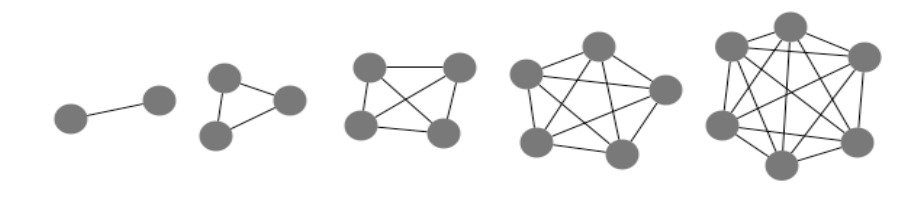
\includegraphics[width=0.9\linewidth]{CommunicationComplexity.png}
    \caption{Overview of communication channel complexity}
    \label{fig:communication-complexity}
\end{figure}

One of the primary challenges is that communication complexity grows with team size and gets considerably more challenging when the team is distributed. As a result, large groups are implicitly conduits for poor communication. The complexity of the channel increases nonlinearly as the number of the team members grows. A three-person team has three communication channels, while a five-person team has ten, or double the number of people. This is represented in Fig.~\ref{fig:communication-complexity}. ~\cite{refpaper6}. As a result, appropriate synchronous communication channels are needed to carry out communication in efficient manner. In one of the case studies, it is mentioned that a startup called Snowpatrol used Skype to conduct synchronous communication in order to minimize the time to market for the product introduction. They used Skype for meetings and used its chat feature extensively in their daily activities. They employed chat channels for various themes, resulting in an efficient communication system. Ad hoc chats addressed unique work difficulties, promoting speedy and concentrated talks among distant team members.~\cite{refpaper7} The first case study depicts how SkypeTM is integrated into people's work practices in an academic setting, and how it has an immediate impact on managerial practices. In Case Study 1, with its adaptable frameworks, SkypeTM enables team members to contact their manager, Karl, as needed, ensuring a collaborative and flexible approach. It demonstrates how SkypeTM improves interaction quality and promotes independent work.~\cite{refpaper7}. In contrast, the second scenario discussed how telecommuting and project-related travel could foster a distributed work environment even when the team is based in one location.  Manager Martin has established communication guidelines for updating activities and their locations as a result. Because of this non-traditional usage of SkypeTM, there was more transparency, which made it easier for everyone to comprehend each other's responsibilities and allowed for the application of standard managerial procedures for control and coordination. Finally, using speech bubbles can aid in efficiently doing activities.~\cite{refpaper7}

\subsection{Approach 3}
In this case study, a research was conducted to use Facebook for multichannel chats for development of web based product for 3 universities in Pakistan. The study revolves around understanding the aspects  influencing channel choice, team composition, data collection methods supported by qualitative and quantitative analysis methods, including social network analysis, emotion analysis, and socio-technical congruence, to draw insights into team dynamics, communication patterns, and coordination effectiveness. ~\cite{refpaper8}

\section{Findings \& Conclusions}

\begin{itemize}
    \item According to approach 1, Computer Mediated Asynchronous Communicaiton has helped us how we pursue teamwork, communicaiton and decision making. CMAC teams can communicate, share information, and make decisions in the context of distributed work environment.CMAC teams are easily scalable, allowing for the inclusion of more professionals or the creation of subteams as needed. This flexibility makes it possible for team members to easily share conversations and information electronically, do research, and consult other experts. ~\cite{refpaper5}\\
    \item As per approach 2, Skype offered numerous people a way to communicate with CMC. It is an easy and dependable method of conducting synchronous communication. As a result, the range of functions offered does not dictate how it is used. Instead, how it is used and how big of an influence it has depends on how the technology is appropriated. The case studies highlight innovative approaches that have developed around SkypeTM or that SkypeTM has integrated into. supporting the transcendence of temporal and spatial limitations and providing more detail on the concepts of awareness, availability, and presence. Rich evidence of intricate patterns of technology interpretation, adoption, appropriation, embedding, and enactment, influenced by social practices, management cultures, and organizational structures, was presented by the examples. ~\cite{refpaper7}\\
    \item According to approach 3, the study's findings indicate that companies in developing nations may find it advantageous to use explicit channels such as Facebook for team coordination and communication in a distributed work environment. Notwithstanding certain privacy and confidentiality issues, these might be resolved by implementing Facebook's security features. ~\cite{refpaper8}
\end{itemize}

    \begin{thebibliography}{8}
        \bibitem{reficon1}
        “Free Icons,” Icons8.com, 2019. \url{https://icons8.com/icons}
        \bibitem{refbook1}
        97 Things Every Engineering Manager Should Know [Book],” www.oreilly.com. \url{https://www.oreilly.com/library/view/97-things-every/9781492050896/}
        \bibitem{refpaper1}
        E. Coiera, “Communication systems in healthcare,” The Clinical biochemist. Reviews, vol. 27, no. 2, pp. 89–98, 2006, \url{https://www.ncbi.nlm.nih.gov/pmc/articles/PMC1579411/} 
        \bibitem{refarticle1}
        What is Asynchronous Communication and How Do Teams Use It?,”\url{https://www.betterup.com/blog/asynchronous-communication}
        \bibitem{refpaper2}
        S. E. Mair, "Two Conversations for One: Synchronous Multimodal Communication," Georgetown University, ProQuest Dissertations Publishing, 2020, 28091233
        \bibitem{refpaper3}
        B.A.Nardi, J.Schiano, M.Gumbrecht, and L.Swartz, "Communication, collaboration,and bugs: the social nature of issue tracking in small,collocated teams", Proceedings of the 2010 ACM conference on Computer supported cooperative work, 2010, pp.291–300, \url{https://dl.acm.org/doi/10.1145/1718918.1718972}
        \bibitem{refpaper4}
        Kumar, Anil and Natarajan, Subhashree and Acharjya, Biswajit. (2017). Computer mediated communication: A pathway to analyze social media communication trajectories. Man in India. 97. 195-205.
        \bibitem{refpaper5}
        Berry, G. R. (2006). Can Computer-Mediated Asynchronous Communication Improve Team Processes and Decision Making? Learning From the Management Literature. The Journal of Business Communication (1973), 43(4), 344-366. \url{https://doi.org/10.1177/0021943606292352}
        \bibitem{refpaper6}
        Lalsing, Vikash, Somveer Kishnah, and Sameerchand Pudaruth. "People factors in agile software development and project management." International Journal of Software Engineering \& Applications 3.1 (2012): 117.
        \bibitem{refpaper7}
        Seeber, I., Maier, R., Ceravolo, P., \& Frati, F. (2014). Tracing the development of ideas in distributed, IT-supported teams during synchronous collaboration
        \bibitem{refpaper8}
        Ferdous, Sehrish, and Naveed Ikram. Communication and Coordination Using Facebook: A Case Study of Distributed Software Development." Journal of Information Science \& Engineering 33.6 (2017)
    \end{thebibliography}
    
\end{document}
